\documentclass{article}
\usepackage[T1]{fontenc}
\usepackage{lmodern}
\usepackage{graphicx}
\usepackage{amsmath,amssymb}
\usepackage[a4paper,margin=2cm]{geometry}
\usepackage[absolute,overlay]{textpos}
\setlength{\TPHorizModule}{1mm}
\setlength{\TPVertModule}{1mm}
\usepackage[indonesian]{babel}
\usepackage{hyperref}
\setlength{\emergencystretch}{2em}
% unit: Halaman 30

\begin{document}

% === Halaman 30 (llm) ===

\vspace{87.91mm}

Contoh:\vspace{10mm}

% deskripsi: Operasi penjumlahan dua matriks berukuran 4x4 dengan elemen heksadesimal yang menghasilkan matriks hasil penjumlahan.
% bbox normalisasi: [0.1040, 0.3010, 0.9080, 0.5970]
\begin{textblock*}{168.84mm}(21.84mm,89.40mm)
\noindent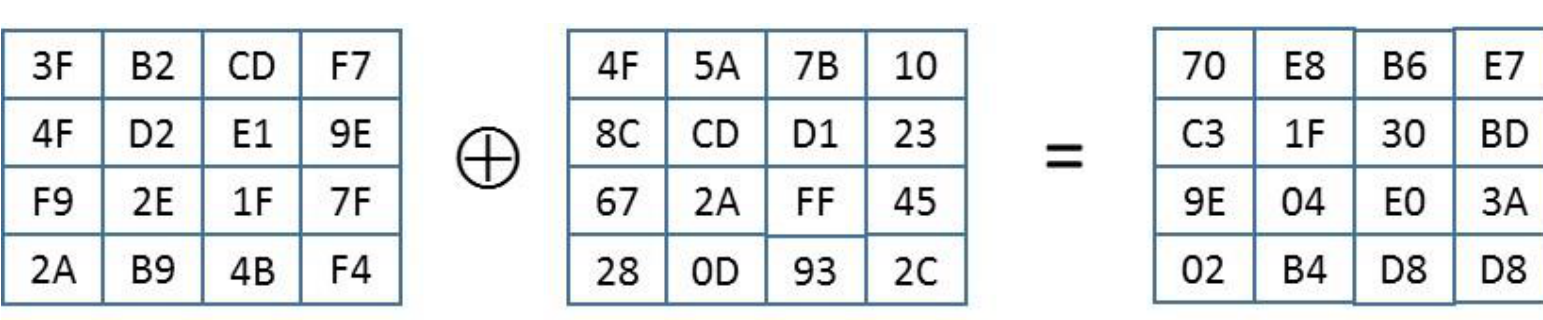
\includegraphics[width=168.84mm,height=87.91mm]{../../images/llm/page_030_img_01.png}%
\end{textblock*}

\end{document}
